\documentclass[a4paper,12pt]{report}
\usepackage{graphicx}  % For including graphics
\usepackage{hyperref}  % For hyperlinks
\usepackage{listings}  % For code snippets
\usepackage{tocbibind} % For adding ToC to the table of contents
\usepackage{titlesec}  % For customizing titles
\usepackage[ngerman]{babel}
\usepackage{wasysym}


\usepackage{geometry}
\geometry{
    top=1in,
    left=1in,
    right=1in,
    bottom=1in
}


\titleformat{\chapter}[block]   % Set chapter format to block style (both on same line)
{\normalfont\huge\bfseries}     % Format for the chapter number and title
{\thechapter}                   % Shows the chapter number followed by a dot
{0.5em}                         % Space between the chapter number and title
{}                              % Formatting for the chapter title (leave empty)

\renewcommand{\contentsname}{Inhaltsverzeichnis}
\renewcommand{\listtablename}{Tabellenverzeichnis}
\renewcommand{\listfigurename}{Abbildungsverzeichnis}
\renewcommand{\lstlistlistingname}{Code-Ausschnitte}
\renewcommand{\abstractname}{Zusammenfassung}
\renewcommand{\chaptername}{Kapitel}

\begin{document}

% Title Page
    \begin{titlepage}
        \centering
        \textit{Berner Fachhochschule}\\[0.2em]
        \textit{BTI3031 Project 1}
        \vfill
        {\huge \textbf{AI-Aided Caches-n-Logs Monitoring-n-Wiping Daemon}}\\[4em]
        {\large Luca Scherer, Janic Scherer, Luca Ammann }\\[0.5em]
        \begin{tabular}{ll}
            \textbf{Betreuer:}\hspace{0.5em}Dr. Simon Kramer \\
        \end{tabular}

        \vfill
        \textit{\today}
    \end{titlepage}

% Abstract
    \begin{abstract}
        \ldots
    \end{abstract}

% Table of Contents
    \tableofcontents
    \listoftables
    \listoffigures
    \lstlistoflistings

% Main Content


    \chapter{Einleitung}


    \section{Ausgangssituation}


    \section{Projektziel}


    \section{Prioritäten}


    \chapter{Spezifikation}

    \newpage
    \section{Systemabgrenzung}

    \subsection{Systemumgebung}

    \subsubsection{Komponenten}


    \begin{figure}[h]
        \centering
        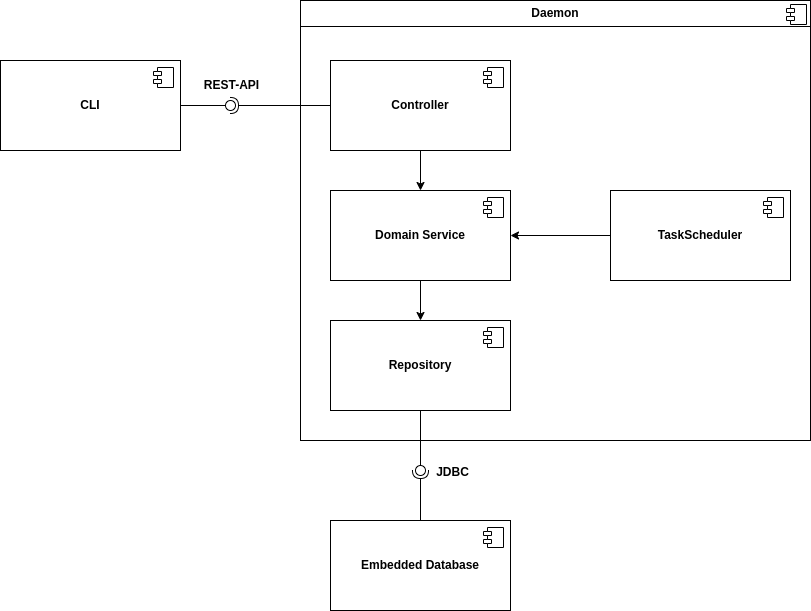
\includegraphics[width=1\textwidth]{assets/comp-diag-aclom}
        \caption{UML Komponentendiagramm}
        \label{fig:comp-diag}
    \end{figure}

    \textnormal{Das System besteht aus zwei Hauptkomponenten, welche als eigene Laufzeiteinheiten ausgeführt werden.
    Die CLI wird ad hoc gestartet und dient als Benutzerschnittstelle.
    Der Daemon läuft nach dem Start im Hintergrund und führt periodisch Befehle aus. Ausserdem stellt er der
    CLI eine REST-Schnittstelle zur Verfügung.
    Ein eingebettetes Datenbanksystem speichert die Applikationsdaten.}

    \begin{table}[h!]
        \centering
        \setlength{\leftmargini}{0.4cm}
        \begin{tabular}{|p{2.5cm}|p{5.5cm}|p{3cm}|}
            \hline
            \textbf& \textbf{Zweck} & \textbf{Technologien (primär)} \\
            \hline
            \textbf{CLI} & {Stellt eine Kommandozeilen-Benutzerschnittstelle zur Verfügung.} & Java, Spring (Shell) \\
            \hline
            \textbf{Controller} & Implementiert die Endpunkte der REST-Schnittstelle & Java, Spring (Data) \\
            \hline
            \textbf{Domain Service} & Applikationslogik & Java, Spring \\
            \hline
            \textbf{Task Scheduler} & Führt Funktionen periodisch aus & Java, Spring \\
            \hline
            \textbf{Repository} & Stellt den Zugang zu den persisiterten Daten zur Verfüfung & Java, Spring (Data) \\
            \hline
            \textbf{Embedded Database} & Speichert Applikationsdaten & SQLite \\
            \hline
        \end{tabular}
        \caption{Beschreibung der Komponenten}\label{tab:table3}
    \end{table}

    \newpage

    \subsection{Prozessumgebung}

    \newpage
    \section{Anforderungen}
    Die Anforderungen für den AI-Aided Caches-n-Logs Monitoring-n-Wiping Demon ergaben sich aus dem Projekt Proposal sowie einem initialen Termin mit Herr Kramer.

    \subsection{Funktionale Anforderungen}

    Alle funktionalen Anforderungen werden in Form von User Stories im Scrum Product Backlog geführt. Dieser wird laufend erweitert beziehungsweise konkretisiert. Eine User Story gilt erst als abgeschlossen, sobald alle dazugehörende Akzeptanzkriterien erfüllt sind. Folgende funktionale Anforderungen wurden definiert und in User Stories inkl. Akzeptanzkriterien abgebildet:
    \begin{itemize}
        \item Das System findet jegliche Log- oder Cache-Dateien, welche sich in einem angegebenen Verzeichnis befinden. Dabei werden auch alle Unterverzeichnisse berücksichtigt.
        \item Das System durchsucht periodisch angegebene Verzeichnisse inkl. Unterverzeichnisse nach Log- oder Cache-Dateien.
        \item Das System erstellt periodisch sogenannte Snapshots der gefundenen Dateien, um diese später miteinerander zu vergleichen.
        \item Das System identifiziert veränderte Dateien anhand der periodisch erstellten Snapshots.
        \item Das System kann den Verwendungszweck von angegebenen Dateien erkennen und nach folgenden Merkalen kategorisieren oder bewerten:
        \begin{itemize}
            \item Dateityp
            \item Verwendungszweck
            \item Schädlichkeit
            \item Leer- bzw. löschbar
        \end{itemize}
        \item Das System kann angegebene Dateien, nach einer Bestätigung des Benutzers leeren oder löschen.
    \end{itemize}
    TODO: Backlog einbinden/beschreiben

    \newpage
    \subsection{Grenz- und Vorbedingungen}
    Im Scrum Product Backlog werden nichtfunktionalen Anforderungen bzw. Grenz- oder Vorbedingungen nicht explizit als User Story geführt. Aus dem Projekt-Proposal und dem initialen Termin ergaben sich nachfolgende nichtfunktionale Anforderungen.
    Diese beeinflussten massgeblich die Architektur des Systems. Keine User Story darf eine oder mehrere nichtfunktionale Anforderungen verletzten, was durch die Definition of Done sichergestellt und laufend geprüft wird.

    \begin{table}[h!]
        \centering
        \setlength{\leftmargini}{0.4cm}
        \begin{tabular}{|c|p{10cm}|}
            \hline
            \textbf{ID} & NFR-001 \\ \hline
            \textbf{Anforderung} & Hintergrundprozess mit periodischem Task (deamon) \\ \hline
            \textbf{Beschreibung} & Das System muss einen Hintergrundprozess implementieren, der periodisch Aktionen durchführen kann. \\ \hline
            \textbf{Akzeptanzkriterien} &
            \begin{itemize}
                \item Nach dem Start des Prozesses, ist dieser für den Benutzer nicht mehr ersichtlich.
                \item Der Hintergrundprozess ist erweiterbar, sodass dieser periodisch und autonom Aktionen durchführen kann.
            \end{itemize}
            \\ \hline
        \end{tabular}
        \caption{Nichtfunktionale Anforderung NFR-001}\label{tab:table}
    \end{table}

    \begin{table}[h!]
        \centering
        \setlength{\leftmargini}{0.4cm}
        \begin{tabular}{|c|p{10cm}|}
            \hline
            \textbf{ID} & NFR-002 \\ \hline
            \textbf{Anforderung} & Benutzerschnittstelle via Konsole (CLI) \\ \hline
            \textbf{Beschreibung} & Mit dem laufenden deamon soll via Konsole interagiert werden können. \\ \hline
            \textbf{Akzeptanzkriterien} &
            \begin{itemize}
                \item Der deamon kann via CLI gestartet werden.
                \item Alle Konfigurationen und Aktionen des deamon sind via CLI verfügbar
            \end{itemize}
            \\ \hline
        \end{tabular}
        \caption{Nichtfunktionale Anforderung NFR-002}\label{tab:table4}
    \end{table}

    \begin{table}[h!]
        \centering
        \setlength{\leftmargini}{0.4cm}
        \begin{tabular}{|c|p{10cm}|}
            \hline
            \textbf{ID} & NFR-003 \\ \hline
            \textbf{Anforderung} & Systemunabhängigkeit \\ \hline
            \textbf{Beschreibung} & Lauffähigkeit mit vollem Funktionsumfang auf gängigen Betriebssystemen. \\ \hline
            \textbf{Akzeptanzkriterien} &
            \begin{itemize}
                \item Hintergrundprozess sowie Konsolenschnittstelle sind auf allen gängigen Betriebssystemen lauffähig und mit vollem Funktionsumfang verwendbar.
                \item Neuimplementierte Features werden auf aktuellen Versionen von Windows, Linux (Ubuntu) und MacOS getestet.
            \end{itemize}
            \\ \hline
        \end{tabular}
        \caption{Nichtfunktionale Anforderung NFR-003}\label{tab:table5}
    \end{table}

    \begin{table}[h!]
        \centering
        \setlength{\leftmargini}{0.4cm}
        \begin{tabular}{|c|p{10cm}|}
            \hline
            \textbf{ID} & NFR-004 \\ \hline
            \textbf{Anforderung} & Codequalität \& erweiterbare Architektur \\ \hline
            \textbf{Beschreibung} & Minimaler, modularer und selbserklärender Code  \\ \hline
            \textbf{Akzeptanzkriterien} &
            \begin{itemize}
                \item Die Architketur wird so aufgebaut, dass neue Features problemlos ergänzt werden können. (z.B. GUI)
                \item Tests gemäss Testkonzept.
                \item Statische Analysen zeigen keine schwerwiegenden verstösse gegen Linting-Regeln.
                \item Anwendungen von gängigen Design-Prinzipen vie SOLID, DRY, KISS etc.
                \item Für jede Codeerweiterung wird eine Codereview durch einen zweiten Entwickler vorgenommen.
            \end{itemize}
            \\ \hline
        \end{tabular}
        \caption{Nichtfunktionale Anforderung NFR-004}\label{tab:table6}
    \end{table}

    \clearpage
    \subsection{Testkonzept}
    \subsubsection{Ziel des Testkonzepts}
    \begin{itemize}
        \item Sicherstellen, dass das gesamte System stabil läuft und seine Hauptfunktionen zuverlässig verfügbar sind.
        \item Minimales Testing-Setup, das nur dort Unit-Tests verwendet, wo es Sinn ergibt (z. B. kritische Algorithmen), um den Entwicklungsaufwand gering zu halten.
        \item Fokus auf Integrationstests und funktionale Tests zur Überprüfung der gesamten Systemfunktionalität.
        \item Klare Definition, welche Tests während der Entwicklung (Teil einer User Story) umgesetzt werden sollen.
    \end{itemize}

    \subsubsection{Testarten und Testabdeckung}
    \begin{itemize}
        \item \textbf{Unit-Tests}: Nur für kritische, isolierbare Logiken wie:
        \begin{itemize}
            \item \textbf{Hash-Algorithmen}: Test der Konsistenz und Korrektheit, insbesondere, wenn Hashes fürs  Verzeichnis Monitoring verwendet werden.
            \item \textbf{File-Suche}: Suchalgorithemen für Log- oder Cache-Dateien.
        \end{itemize}
        \item \textbf{Integrationstests}: Testen der Zusammenarbeit mehrerer Komponenten.
        \begin{itemize}
            \item \textbf{CLI-Befehle}: Überprüfen, dass die CLI-Kommandos (\texttt{run}, \texttt{search}) korrekt ausgeführt werden und die erwarteten Parameter validieren.
            \item \textbf{REST-HTTP-Anfragen}: Testen, ob alle HTTP-Schnittstellen korrekt reagieren. (Happy- sowie Exception-Paths)
        \end{itemize}
        \item \textbf{End-to-End Tests}: Fokus auf End-to-End-Szenarien zur Validierung der zentralen Funktionalität.
    \end{itemize}

    \subsubsection{Test-Setup und -Konfiguration}
    \begin{itemize}
        \item \textbf{Mocking von Ressourcen}: Verwenden von Mocks für Datenbank- und Dateisystemzugriffe in den Unit-Tests, um sie isoliert zu halten.
        \item \textbf{Testumgebung}: Erstellen einer dedizierten Test-DB und eines Testverzeichnisses.
        \item \textbf{Automatisierte Testausführung}: Integration der Tests in die CI/CD-Pipeline, um sicherzustellen, dass das System stabil bleibt.
    \end{itemize}

    \clearpage
    \section{Usability}\label{sec:usability}

    \subsection{Personas}\label{subsec:personas}

    \subsubsection{Thomas}

    \begin{figure}[h]
        \centering
        
\includegraphics[width=0.6\textwidth]{assets/persona1}
        \caption{Thomas \footnote}
        \label{fig:persona-1}
    \end{figure}


    Thomas ist ein 35-Jähriger Berufsschullehrer, der Informatiker und Elektroniker unterrichtet.
    Für seine Schüler unterrichtet er unter anderem auch
    Systemadministration und IT-Sicherheit.
    Thomas ist sehr interessiert an neuen Technologien und probiert gerne neue Software aus.
    Daher stellt er sich die Frage, warum so viele Log- und Cache-Dateien auf seinem Rechner sind, ob diese alle
    ihre Daseinsberechtigung haben und auch ob das Lesen und Schreiben dieser Dateien nicht ein Sicherheitsrisiko
    darstellt.
    Thomas ist ein sehr erfahrener Benutzer und hat keine Probleme mit der Kommandozeile.

    \begin{table}[h!]
        \centering
        \setlength{\leftmargini}{0.4cm}
        \begin{tabular}{|p{2.5cm}|p{7cm}|}
            \hline
            \textbf Aufgaben & KnowHow stärken (in Bezug auf seine Lehrtätigkeiten) \\
            \hline
            \textbf Ziele & Veränderungen beobachten können und diese überprüfen lassen \\
            \hline
            \textbf Wünsche & Intuitive Benutzerschnittstelle \\
            \hline
            \textbf Hindernisse & Trotz Erfahrung in der Informatik, sind teilweise Wissenslücken vorhanden \\
            \hline
        \end{tabular}
        \label{tab:table7}
    \end{table}

    \footnotetext{\url{https://www.pexels.com/de-de/foto/mann-arbeiten-tippen-pc-16129724/}.}


    \newpage
    \subsection{Storyboard}

    \subsection{UX-Prototyping}


    \chapter{Implementierung}


    \section{Architektur}


    \section{Prozesse}
    \url{https://www.ganttlab.com} \\
    \url{https://www.hermes.admin.ch/de/projektmanagement/verstehen/ubersicht-hermes/methodenubersicht.html}


    \chapter{Bereitstellung/Integration}

    \begin{figure}[h]
        \centering
        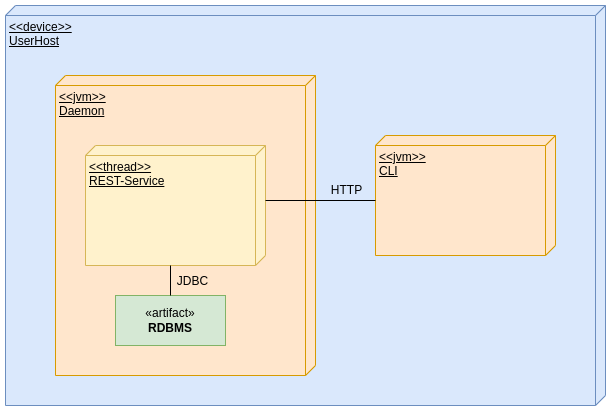
\includegraphics[width=1\textwidth]{assets/DeplDiagram}
        \caption{UML Deploymentdiagramm}
        \label{fig:depl-diag}
    \end{figure}

    Das ganze System befindet sich während der Laufzeit auf dem Host-Gerät des Anwenders.
    Dazu werden zwei separate jar-Dateien ausgeliefert.
    Das Erste sollte bereits beim Start des Geräts ausgeführt werden und die JVM für den Daemon starten.
    Dieser startet einen Webservice, der REST-Schnittstellen für die Steuerung des Daemons anbietet.
    Dieser REST-Service kommuniziert ausserdem über JDBC mit einem RDBMS, welches in Form von einer einzigen Datei (SQLite)
    im Daemon embedded ist.

    Das zweite jar sollte dann manuell vom Anwender gestartet werden sobald er Funktionen des Daemons ausführen möchte.
    Dieses jar startet wiederum eine zweite jvm, welche ein CLI für den Anwender mit bestimmten Kommandos zur Verfügung stellt.
    Diese CLI sendet dann über HTTP die entsprechenden Anfragen an den Daemon, die zur Erfüllung der Anweisungen des Anwenders führen.


    \section{Lizenzierung}


    \section{Installationshandbuch \& Skript}


    \section{Benutzerhandbuch}


    \chapter{Fazit}


    \section{Diskussion}


    \section{Zusammenfassung}


    \section{Zukünftige Arbeiten}
    \url{https://doi.org/10.1145/3664811}


    \chapter{Glossar}


    \chapter{Index}


    \chapter{Bibliografie}


    \chapter{Anhang}


    \section{Facsimile der Projektbeschreibung}


    \section{Erklärung zur Urheberschaft}

\end{document}
